% Task 2 -- Niederer cardiac benchmark + ECG. Compile: pdflatex (x2) in this dir.
\documentclass[aspectratio=169,10pt]{beamer}
\usepackage[T1]{fontenc}\usepackage{lmodern}\usepackage{amsmath,amssymb,bm}
\usepackage{booktabs}\usepackage{graphicx}\graphicspath{{./}}
\definecolor{Struct}{HTML}{1F3A5F}\definecolor{Gray}{HTML}{6E6E6E}\definecolor{Accent}{HTML}{8C2D04}
\usetheme{default}\usefonttheme{professionalfonts}\setbeamertemplate{navigation symbols}{}
\setbeamercolor{structure}{fg=Struct}\setbeamercolor{frametitle}{fg=Struct}
\setbeamerfont{frametitle}{series=\bfseries,size=\large}
\setbeamercolor{block title}{fg=white,bg=Struct}\setbeamercolor{block body}{bg=Struct!6}
\setbeamertemplate{frametitle}{\vskip0.4em\hspace{0.2em}\usebeamerfont{frametitle}\insertframetitle%
  {\ifx\insertframesubtitle\empty\else\\[0.1em]\small\color{Gray}\insertframesubtitle\fi}\par}
\setbeamertemplate{footline}{\hfill\footnotesize\color{Gray}\insertframenumber\,/\,\inserttotalframenumber\hspace{0.4cm}\vspace{3pt}}
\renewcommand{\arraystretch}{1.15}
\begin{document}

\begin{frame}[plain]\vskip1.0cm
{\color{Struct}\large\bfseries Task 2 --- Niederer cardiac benchmark + ECG (PETSc, this machine)\par}
\vskip0.4em{\color{Gray} TP06 monodomain on the $20{\times}7{\times}3$ mm slab $\to$ pseudo-ECG\par}
\vskip0.8em\hrule height0.4pt\vskip0.5em\footnotesize
\texttt{asm\_bug\_demo/cardiac/}: \texttt{tt06.h}, \texttt{tt06\_cell.c}, \texttt{monodomain.c}.
\end{frame}

\begin{frame}{Problem definition --- the exact example}
\framesubtitle{Niederer et al.\ (2011) benchmark; cell model ten Tusscher--Panfilov 2006 (epi)}
\begin{itemize}\itemsep0.25em\small
  \item \textbf{Heart}: $20{\times}7{\times}3$ mm slab, fiber $\|x$; $h{=}0.5$ mm; $\Delta t{=}0.02$ ms.
  \item \textbf{Monodomain}: $\chi(C_m\partial_tV_m+I_{\rm ion})=\nabla\!\cdot(\bm\sigma\nabla V_m)+I_{\rm stim}$, zero-flux boundary.
  \item \textbf{Params}: $\chi{=}140/\mathrm{mm}$, $C_m{=}0.01\,\mu\mathrm F/\mathrm{mm}^2$, $\sigma_L{=}0.1334$, $\sigma_T{=}0.0176$ mS/mm.
  \item \textbf{Stimulus}: $1.5^3$ mm cube at the $(0,0,0)$ corner, 2 ms.
  \item \textbf{Discretization (cardiac.pdf)}: P1 lumped-mass FEM; \textbf{IMEX} Crank--Nicolson diffusion ($=$ \textbf{Sys 1} $\tfrac{\chi C_m}{\Delta t}M+\tfrac12K_\sigma$) $+$ explicit reaction; Rush--Larsen gating $+$ FE concentrations.
  \item \textbf{ECG}: lead-field pseudo-ECG. (Full torso Sys 2/Sys 3 built in Task 3.)
\end{itemize}
\end{frame}

\begin{frame}{Stage 1 --- TP06 single cell: verified action potential}
\begin{center}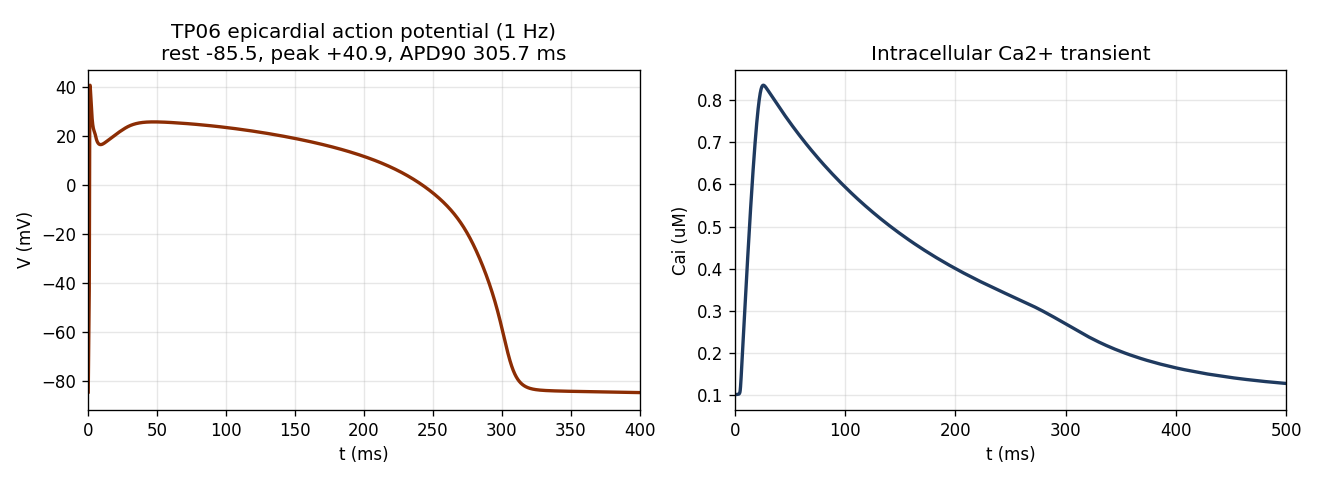
\includegraphics[width=0.86\textwidth]{fig_tt06_ap}\end{center}
\vskip-0.2em\footnotesize
Resting \textbf{$-85.5$ mV}, peak \textbf{$+40.9$ mV}, \textbf{APD90 $305.7$ ms} (all physiological);
correct spike--dome--plateau (Ito notch) and Ca$^{2+}$ transient ($\sim0.84\,\mu$M). The ionic foundation is correct.
\end{frame}

\begin{frame}{Stage 2 --- monodomain propagation + mesh convergence}
\begin{center}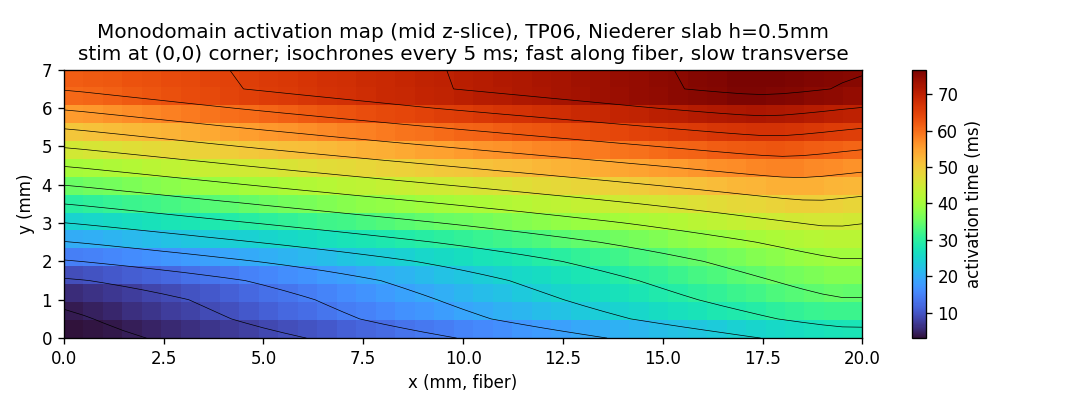
\includegraphics[width=0.82\textwidth]{fig_mono_activation}\end{center}
\vskip-0.2em\footnotesize
Anisotropic spread from the corner (fast along fiber, slow transverse; elliptical isochrones, 5 ms).
\textbf{Mesh convergence (the benchmark's point):} far-corner P8 $76.5$ ms ($h{=}0.5$) $\to$ $\mathbf{47.6}$ \textbf{ms} ($h{=}0.2$),
toward the Niederer consensus $\sim$43 ms. Longitudinal CV $\approx0.96$ m/s (mesh-stable, same order as 0.6--0.7).
\end{frame}

\begin{frame}{Stage 3 --- ECG: QRS + T-wave}
\begin{center}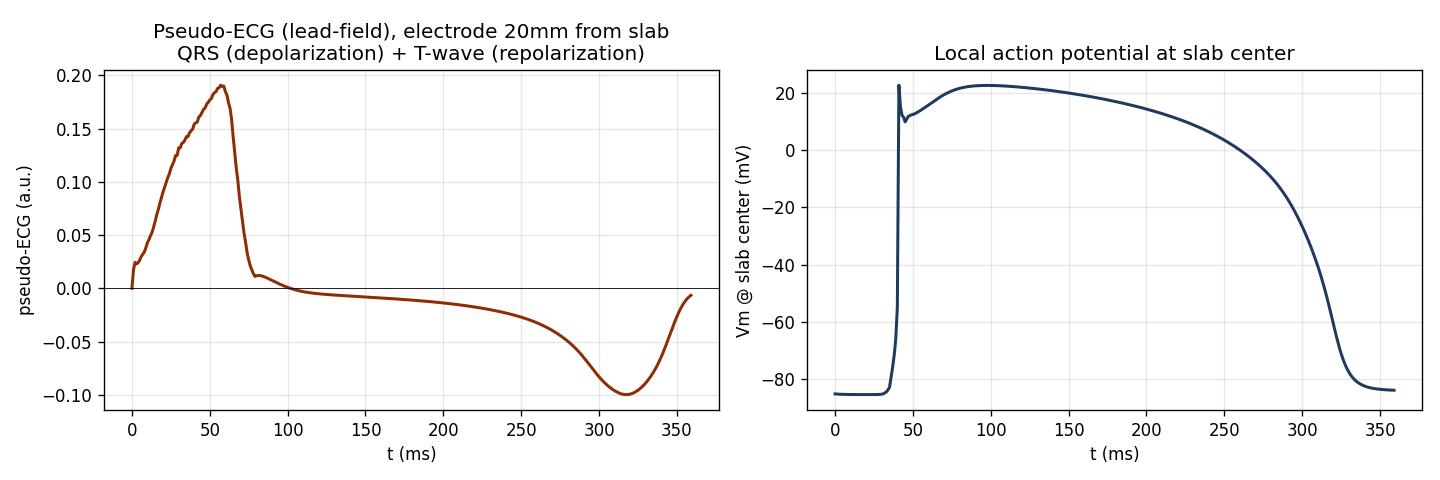
\includegraphics[width=0.95\textwidth]{fig_mono_ecg}\end{center}
\vskip-0.2em\footnotesize
Full beat (360 ms): positive \textbf{QRS} (depolarization, peak $\sim$57 ms) $\to$ baseline $\to$ negative \textbf{T-wave}
(repolarization, trough $\sim$315 ms), consistent with the AP duration. Recognizable ECG morphology.
\end{frame}

\begin{frame}{Verification summary (Task 2)}
\begin{block}{End-to-end pipeline VERIFIED}
\footnotesize
\begin{tabular}{l ll l}
\toprule
 & this implementation & Niederer consensus & \\
\midrule
TP06 rest / peak / APD90 & $-85.5$ / $+40.9$ / $305.7$ ms & $\sim-85$ / $\sim+40$ / $\sim280$ ms & \checkmark \\
P8 far-corner ($h{=}0.2$) & 47.6 ms & $\sim$42.9 ms & within $\sim$10\%, converging \\
longitudinal CV & 0.96 m/s & 0.6--0.7 m/s & same order \\
ECG morphology & QRS$(+)\to$T$(-)$ & QRS$\to$T & \checkmark \\
\bottomrule
\end{tabular}
\end{block}
\vskip0.2em
\begin{itemize}\itemsep0.2em\footnotesize
  \item TP06 cell $\to$ anisotropic monodomain (converges to the consensus under refinement) $\to$ ECG (QRS$+$T): \textbf{the pipeline is correct}.
  \item Honest: CV slightly fast (finer mesh $+$ $\sigma$ tuning would tighten it; codes differ $\sim$10--20\%). The full torso forward (Sys 2 recover $+$ Sys 3 torso) is built in Task 3.
\end{itemize}
\end{frame}

\end{document}
